\documentclass[12pt]{article}

% This is the preamble, load any packages you're going to use here
\usepackage{physics} % provides lots of nice features and commands often used in physics, it also loads some other packages (like AMSmath)
\usepackage{siunitx} % typesets numbers with units very nicely
\usepackage{enumerate} % allows us to customize our lists
\usepackage[a4paper, margin=2.5cm]{geometry}
\usepackage[german]{babel}
\usepackage{hyperref}
\usepackage{url}
\usepackage{listings}
\usepackage{xcolor}
\usepackage{graphicx}
\usepackage{sidecap}

\definecolor{codegreen}{rgb}{0,0.6,0}
\definecolor{codegray}{rgb}{0.5,0.5,0.5}
\definecolor{codepurple}{rgb}{0.58,0,0.82}
\definecolor{backcolour}{rgb}{1,1,1}

\lstdefinestyle{mystyle}{
    backgroundcolor=\color{backcolour},   
    commentstyle=\color{codegreen},
    keywordstyle=\color{magenta},
    numberstyle=\tiny\color{codegray},
    stringstyle=\color{codepurple},
    basicstyle=\ttfamily\footnotesize,
    breakatwhitespace=false,         
    breaklines=true,                 
    captionpos=b,                    
    keepspaces=true,                 
    numbers=left,                    
    numbersep=5pt,                  
    showspaces=false,                
    showstringspaces=false,
    showtabs=false,                  
    tabsize=2
}
\lstset{style=mystyle}

\lstdefinelanguage[2]{protobuf}{%
    sensitive=true,%
    morecomment=[l]{//},%
    morecomment=[s]{/*}{*/},%
    morestring=[b]{"},%
    % For the keywords of Protocol Buffers
    % see https://developers.google.com/protocol-buffers/docs/proto
    morekeywords={enum,oneof,map,syntax,public,import,option,package,message,%
        group,optional,required,repeated,default,reserved,extend,extensions,%
        to,max,service,rpc,returns,true,false},%
    % Basic types
    % see https://developers.google.com/protocol-buffers/docs/proto#scalar
    morekeywords=[2]{%
        double,float,int32,int64,uint32,uint64,sint32,sint64,%
        fixed32,fixed64,sfixed32,sfixed64,bool,string,bytes},%
    % Options
    % taken from 'google/protobuf/descriptor.proto'
    morekeywords=[3]{%
        % Generic Options
        deprecated, uninterpreted_option,%
        % File Options
        java_package,java_outer_classname,java_multiple_files,%
        java_generate_equals_and_hash,java_string_check_utf8,optimize_for,%
        go_package,cc_generic_services,java_generic_services,%
        py_generic_services,cc_enable_arenas,obj_class_prefix,%
        csharp_namespace,%
        % Message Options
        message_set_wire_format,no_standard_descriptor_accessor,map_entry,%
        % Field Options
        ctype, packed,jstype,lazy,weak,%
        % Enum Options
        allow_alias}%
}
\lstalias[]{protobuf2}[2]{protobuf}


\begin{document}

\title{%
Convolutional LSTM zur Bewegungsvorhersage von Verkehrsteilnehmern \\
  \large Anwendungen der Künstlichen Intelligenz \\
    Sommersemester 2021}
\author{Armin Straller}
\date{\today}

\maketitle

\begin{abstract}
    Um vorausschauendes Fahren für Autonome Fahrzeuge zu ermöglichen, ist es notwendig die Bewegungen anderer Verkehrsteilnehmer vorherzusagen. 
    Da das Verhalten von Fußgängern, Radfahreren und Autofahrern oft auf Interaktion basiert oder von Ortspezifischen Mustern abhängt, 
    bietet es sich an ein Netzwerk mit historischen Informationen über das Verhalten der Verkehrsteilnehmer aufzubauen.
	Diese Arbeit beschäftigt sich mit einem solchen Netzwerk zur Bewegungsvorhersage von Verkehrsteilnehmern.
    Als Datengrundlage wurde der im Frühjahr 2021 veröffentlichte Waymo Open Motion Datensatz verwendet. 
    Das entwickelte Netzwerk verwendete bildbasierte Eingangsdaten welche eine gerasterte Darstellung der unterschiedlichen Szenarien verwendet.
    Ein LSTM bietet dann die Möglichkeit Daten eines vergangen Zeitraums in Kontext zu bringen und ein eine bildliche Repräsentation eines zukünftigen Zustands auszugeben. 
    Das aus der Arbeit resultierende Netzwerk ermöglicht grundlegende vorhersagen der Bewegungsrichtung ist aber zum aktuellen Entwicklungsstand nicht für den Einsatz in einem Autonomen Fahrzeug geeignet.
\end{abstract}

\section{Problemstellung}
    Die Problemstellung für die entwickelte Künstliche Intelligenz ist aus der Waymo Motion Prediction Challenge abgeleitet.
    Hierbei soll auf Basis der Verkehrsdaten aus einer vergangenen Sekunde eine prädiktion für die folgenden acht Sekunden erfolgen.
    Der dafür bereitgestellte Datensatz ist das Waymo Open Motion Dataset~\cite{ettinger2021large}. 
    Dieses umfasst 574~Stunden und 1750~km an Verkehrsinformation und bietet somit genug Informationen für das Training eines Neuronalen Netzwerks.

    \subsection{Datengrundlage}
        Im Datensatz von Waymo sind verschidene Informationen über die aktuelle Verkehrssituation enthalten. Diese können im Detail dem scenario.proto aus dem Anhang entnommen werden.
        Teil des Scenarios ist auch eine Karte deren Details in der map.proto Datei definiert sind.~\cite{waymo2021github}

        Auf die für diese Arbeit wichtigen Inhalte der Szenarien wird Kapitel über die \hyperref[sec:preprocessing]{Vorverarbeitung der Daten} eingegangen.

\newpage

\section{Related Work und Entstehung der Projektidee}
    Es haben sich bereits andere Arbeiten mit der Vorhersage von Bewegungen im Straßenverkehr beschäftigt. 
    Aufgrund der aktualität des Waymo Datensatzes sind zu diesem allerdings noch keine Veröffentlichungen bekannt. 
    Ein Datensatz mit ähnlichem Inhalt wurde für die Prediktion von anderen Fahrzeugen in der Arbeit von Jeong, Yonghwan verwendet. 
    Hierbei kam ein LSTM-RNN Netzwerk zum Einsatz.~\cite{Yonghwan2020}
    
    Auch die Arbeit von Wu, Jingyuan beschäftigt sich mit der Bewegungsvorhersage. 
    In diesem Fall geht es um Fußgänger und eine Karten- beziehungsweise Modellbasierte Methodik zur Vorhersage. 
    Diese verwendet ein Raster welches die Aufenthaltswahrscheinlichkeit der Fußgänger darstellt.~\cite{Jingyuan2018}

    \subsection{Convolutional LSTM basierte Bewegungsvorhersage}
    Auf Basis der aufgeführten Arbeiten und der zur verfügbaren Daten ist die grundlegende Idee für diese Arbeit entstanden. 
    Die Verkehrsinformationen werden in ein Raster eingetragen und in Bildform als Eingangsdaten für das Convolutional-LSTM verwendet.
    Hierdurch können die Karten- und Positionsdaten der Verkehrsteilnehmer in Relation gebracht werden. 
    Die Historie der Bewegung wird dann durch die Eingangsbreite des LSTMs dargestellt. 
    Das Keras Beispiel "Next-Frame Video Prediction with Convolutional LSTMs"~\cite{Keras2021} dient als Grundlage für die Umsetzung.
    Da das Raster nur mit begrenzter Auflösung arbeitet kann es theoretisch vorkommen, dass das Autonome Fahrzeug 
    im Szenario das Raster verlässt. Um dies zu umgehen wird ein Ansatz eine Transformation des Szenarios in die Ego-Perspektive des autonomen Fahrzeugs beinhalten. 
    Im Folgenden wird daher von einer statischen oder dynamischen Darstellung gesprochen, wobei die dynamische Darstellung die Transformation in die Ego-Perspektive beinhaltet. 

\section{Vorverarbeitung der Daten}
\label{sec:preprocessing}
    Um die Informationen aus dem Waymo Open Motion Dataset in die Darstellungsform des Rasters zu bringen 
    sind einige Schritte notwendig. Diese werden im Folgenden dargestellt. 
    \subsection{Einlesen des Protobuf} 
        Zunächst muss das Szenario aus dem scenario.proto Format eingelesen werden. 
        Hierfür werden Auszüge aus dem Waymo Open Dataset Motion Tutorial~\cite{Tutorial2021} verwendet. 
        Dabei werden allerdings nur die Einträge geladen die für die Rasterisierung der Objekte notwendig sind. 
        Es werden immer alle Zeitschritte geladen und anschließend konvertiert. 
        Dies beinhaltetd die vergangenen, den aktuellen und die zukünftigen Elemente des Protobufs.
    \subsection{Konvertierung der Karte}
        Die Karteninformation ist Teil des scenario.proto und wird in Form des map.proto in jedem Szenario bereitgestellt.
        Ein Auszug aus der map.proto Definition der in Listing~\ref{sec:maplisting} dargestellt wird zeigt diese Liste und die Definition der Punkte. 
        Hierbei ist zu beachten, dass die Punkte in Metern zu einem beliebigen Ursprung gegeben sind. 
        Die "polyline" definiert dann ein Feature des Straßennetzwerks. Diese ist eine Liste von "MapPoints" welche Segemente zwischen aufeinanderfolgenden Punkten definieren.
        Da die Auflösung der Punkt groß genug ist werden diese Einfach in das Raster übertragen. 
        Sobald ein "MapPoint" innerhalb eines Rasterelements liegt wird dieses entsprechend des Linientypen eingefärbt.
        \vspace{0.5cm}
        \begin{lstlisting}[language=protobuf2, caption=Auszug aus map.proto, label={sec:maplisting}]
        repeated MapPoint polyline = 2;
        message MapPoint {
            optional double x = 1;
            optional double y = 2;
            optional double z = 3;
        }
        \end{lstlisting}
        Im folgenden wird die Karte aus dem Szenario %TODO: Insert Scenario Name 
        dargestellt. Die statische Repräsentation das Scenarios erfordert eine einmalige Konvertierung der Karte. 
        Diese bleibt dann für den gesamten Zeitraum des Szenarios konstant.

        \begin{figure}[h]
            \centering
            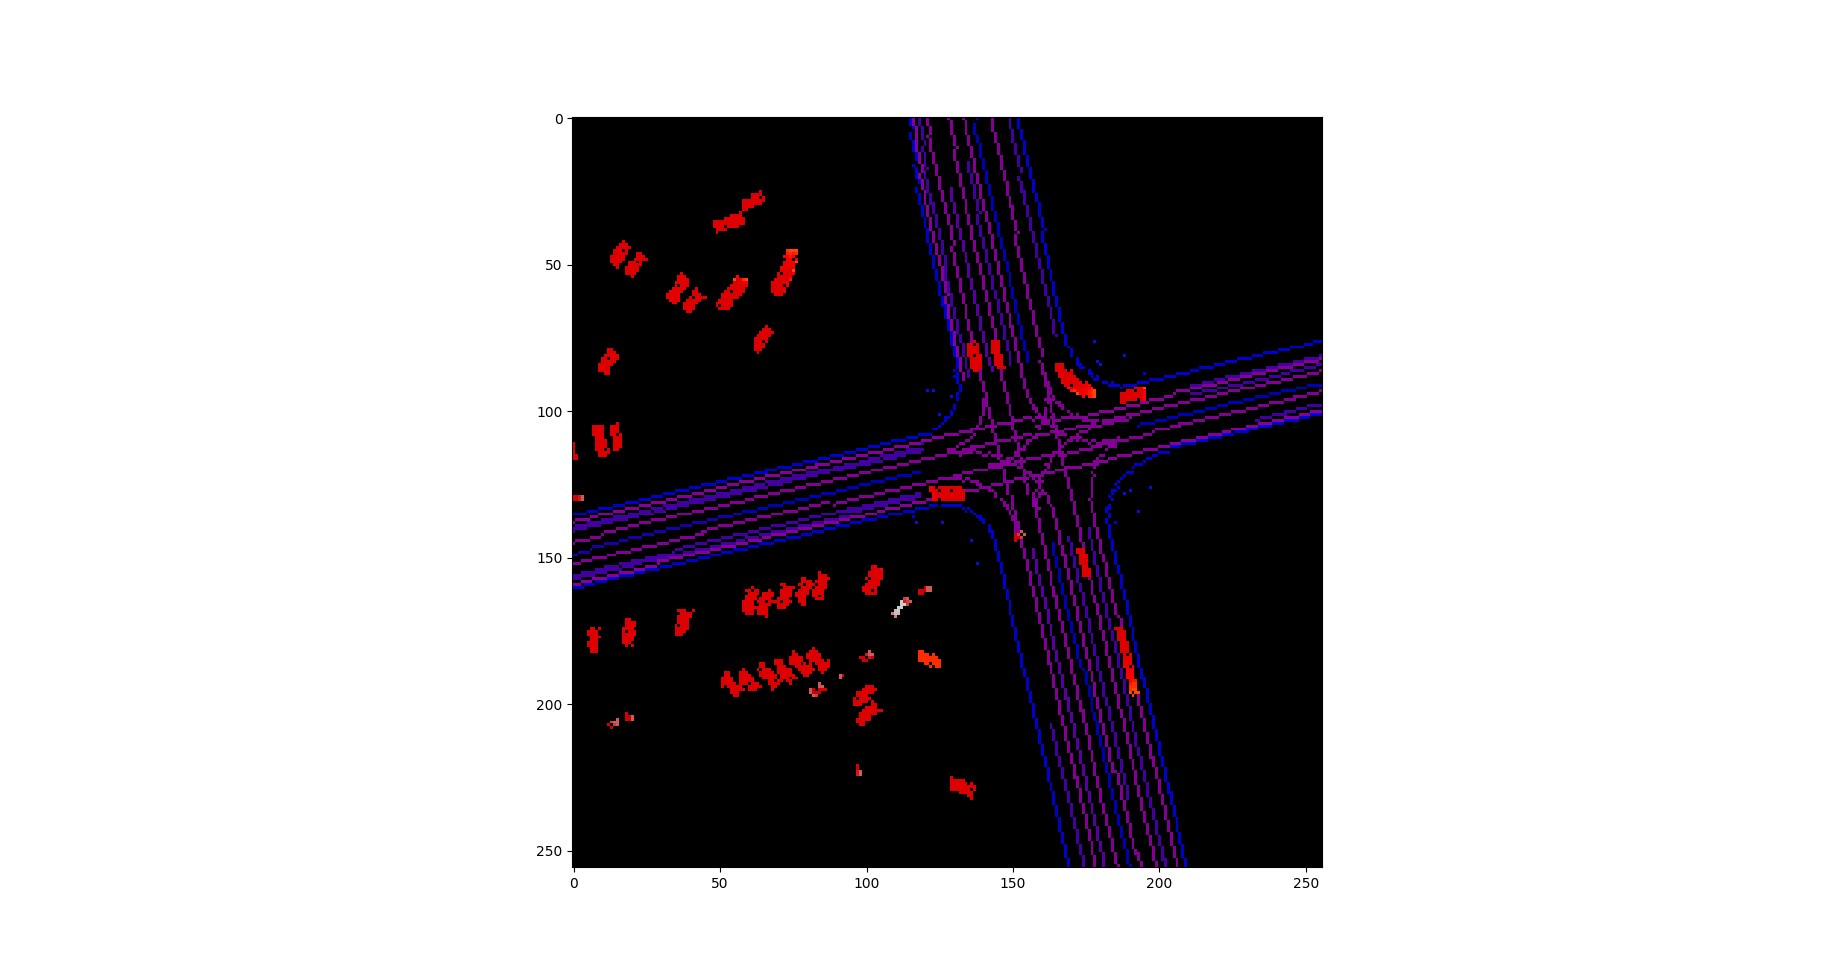
\includegraphics[width=0.8\textwidth]{visu_past_uncompressed_tf_example_training_training_tfexample_tfrecord-00000-of-01000.png}
            \caption{Beispiel einer in das Raster übertragenen Karte}
        \end{figure}

        \paragraph{Dynamische Darstellungsform}
            Für den Fall der dynamischen Darstellung der Karte muss diese bei jeder Bewegung des autonomen Fahrzeugs 
            in dessen Ego-Perspektive transformiert werden. 

        

    \subsection{Konvertierung der Objekte}
        Der Protobuf enthält Informationen über die Größe sowie globale Position und Orienierung der Objekte. 
        Dadurch können die vier 2D-Eckkoordinaten der Objekte berechnet werden. Um diese in das 2D-Raster zu übertragen wird die Grundfläche der Box in 
        zwei Dreiecke aufgeteilt und anschließend Mithilfe des %TODO Algorithms
        in das Raster übertragen. Wenn Objekte kleiner als ein Rasterelement sind, werden sie auf ein ganzes Rasterelement übertragen. 
        So kann sichergestellt werden, dass alle Objekte in der Darstellung repräsentiert werden.

    \subsection{Transformation in dynamische Darstellungsform}


\section{Analysis}
	Here you discuss your observations and results
	
    \subsection{Double Slit Interference}
		The subsection command let's you further divide your sections up.  Comment on your observations and results here
        
        \subsubsection{Varying Parameters}
        	For longer documents, you can even use subsubsections, 
            it's probably overkill for this analysis.
            
            \paragraph{Still More labels}
            	You can also label paragraphs
                
                \subparagraph{Subparagraphs}
                	And even subparagraphs.  Fortunately, we won't be 
                    writing such long documents in this course!
       
       \subsubsection{When to Make New Sections}
        	As a general rule of thumb, don't make smaller sections, subsections, etc, unless there are at least two of them at that level (just like with lists).
	
    \subsection{Single Slit}
		More discussion here
        
\section{Data}
	Please don't include any data tables in your \LaTeX\, write up.  Making tables in \LaTeX\, is very boring, although there are programs to convert your Excel file to \LaTeX\, form!  We'll worry about that later.

\bibliography{motion-prediction}{}
\bibliographystyle{ieeetr}

\end{document}